\documentclass[a4paper,10pt]{article}
\title{CS 349 Assignment 1}
\author{Manan Gupta - 170101035}

\usepackage[shortlabels]{enumitem}
\usepackage[dvipsnames,table]{xcolor}
\usepackage[lmargin=1cm,rmargin=1cm,tmargin=0.5cm,bmargin=1.2cm]{geometry}
\usepackage{tabularx}
\usepackage{graphicx}
\usepackage{calc}
\usepackage{adjustbox}
\usepackage{lipsum}
\usepackage{wrapfig}
\usepackage{subfig}
\usepackage{textcomp}
\usepackage{sectsty}
\chapterfont{\color{blue}}  % sets colour of chapters
\sectionfont{\color{Fuchsia}} 
\newlength{\strutheight}
\settoheight{\strutheight}{\strut}

\makeatletter         
\renewcommand\maketitle{
	{\raggedright {
			\color{RoyalPurple}
		\begin{center}
			{\fontsize{22pt}{22pt} \bfseries \sffamily \@title } \qquad\qquad
			{\fontsize{22pt}{22pt} \bfseries \@author}\\[8ex]
\end{center}}} }
\makeatother
\begin{document}

\maketitle
\vspace{-1cm}
\hrule

\section*{Question 1}
\begin{enumerate}[a)]
	\item \textbf{-c} option is used for specifying the count of ECHO\_REQUESTS to be sent
	\\
	For example :- \textit{\textbf{ping -c 4 10.19.6.44}}. \\
	This command will send 4 ECHO\_REQUESTS to the given address
	\vspace{-0.1cm}\item \textbf{-i} option is used for specifying the time interval between two successive ECHO\_REQUESTS
	\\
	For example :- \textit{\textbf{ping -i 0.5 10.19.6.44}}. \\
	This command will send ECHO\_REQUESTS after every 0.5 seconds.
	\vspace{-0.1cm}\item
	\begin{itemize}
		\item  \textbf{-l} option is used for specifying the number of packets to be sent not waiting for a reply\\
		For example :- \textit{\textbf{ping -l 3 10.19.6.44}}. \\
		This command will send 3 ECHO\_REQUESTS right at the beginning.
		\vspace{-0.1cm}\item The limit for sending such requests for a normal user is \textbf{3}.
	\end{itemize}
	\vspace{-0.1cm}\item
	\begin{itemize}
		\item  \textbf{-s} option is used for specifying the number of data bytes in a packet\\
		For example :- \textit{\textbf{ping -s 32 10.19.6.44}}. \\
		This command will send packets having 32 data bytes.
		\vspace{-0.1cm}\item The total packet size will be \textbf{60 bytes} as 8 bytes of IMCP header and 20 bytes IP header are added.
	\end{itemize}
\end{enumerate}

\section*{Question 2}
\textit{The server is located in New Jersey USA.\\
Time when the readings are taken are \textbf{12:00 am, 7:00 am, 5:00 pm. (Indian Standard Time)}}
\vspace{-0.2cm}
\begin{table}[h]
	\rowcolors{1}{cyan!10}{cyan!20}
	\begin{tabularx}{\textwidth}{|p{85pt}||p{75pt}||p{80pt}||X||X||X||X|}
		\hline
		\rowcolor{cyan!40}
		\textbf{Host Name} & \textbf{IP Address} & \textbf{Location} & \textbf{Latency 1} & \textbf{Latency 2} & \textbf{Latency 3} & \textbf{Avg RTT} \\ \hline
		\textbf{youtube.com}  & 172.217.7.174 & California, USA & 12.074 	ms & 11.640 ms & 11.914 ms & 11.876 ms\\ \hline
		\textbf{web.stanford.edu}  & 171.67.215.200 & Virginia, USA & 66.963 ms & 66.454 ms & 67.507 ms & 66.974 ms\\ \hline
		\textbf{codeforces.com} & 81.27.240.126 & Peterburg, Russia & 121.442 ms & 121.139 ms & 121.896 ms & 121.492 ms\\ \hline
		\textbf{9anime.ru}  & 104.27.157.26 & Illinois, USA & 6.032 ms & 6.105 ms & 6.805 ms & 6.314 ms\\ \hline
		\textbf{hetzner.com} & 78.47.166.55 & Bavaria, Germany & 92.498 ms & 92.486 ms & 93.160 ms & 92.714 ms\\ \hline
		\textbf{blogx.sina.com.cn}& 49.7.37.126 & Beijing, China & 344.783 ms & 334.069 ms & 246.561 ms & 308.471 ms\\ \hline
	\end{tabularx}
	\caption{Round Trip Times for 6 hosts at 3 different times}
\end{table}
\vspace{-0.2cm}
\begin{table}[h]
	\rowcolors{1}{cyan!10}{cyan!20}
	\begin{tabularx}{\textwidth}{|p{130pt}||X||X||X||X||X||X|}
		\hline
		\rowcolor{cyan!40}
		\textbf{Size of Packet} & \textbf{64B} & \textbf{128B} & \textbf{256B} & \textbf{512B}& \textbf{1024B}  & \textbf{2048B} \\ \hline
		\textbf{Latency 1} & 66.963 ms & 67.057 ms & 67.327 ms & 67.201 ms & 67.419 ms & 78.836 ms\\ \hline
		\textbf{Latency 2} & 66.454 ms & 66.503 ms & 66.656 ms & 67.006 ms & 67.582 ms& 78.299 ms\\ \hline
		\textbf{Latency 3} & 67.507 ms & 67.496 ms & 67.531 ms & 67.986 ms & 68.004 ms & 79.383 ms\\ \hline
	\end{tabularx}
	\caption{Round Trip Times for 1 host at 6 different packet sizes}
\end{table}
\begin{enumerate}[a)]
	\begin{adjustbox}{valign=T,raise=\strutheight,minipage={\linewidth}}
		\begin{wrapfigure}{r}{0pt}
			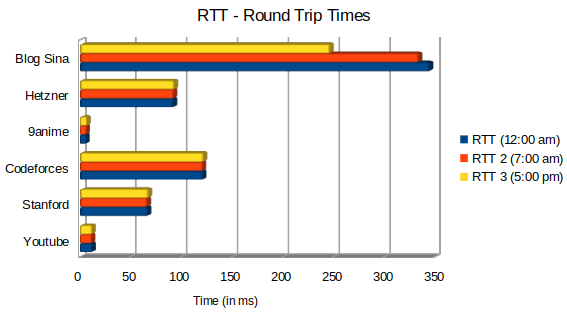
\includegraphics[width=10cm]{rtt1.png}
		\end{wrapfigure}
		\strut{}
		\item
		\textbf{RELATION BETWEEN RTT AND DISTANCE:-} From the observations, we can conclude that RTT and geographical distance are \textbf{weakly correlated}. The relationship can be explained by an \textbf{increased number of hops} required and \textbf{increased propagation delay}. As the distance increases so does the propagation delay. Also, with more distance, more hops are required between nodes which also add \textbf{processing delay} at each node. The relationship is weak as RTT also depends on network traffic and server capacity.
		\item 
		\textbf{PACKET LOSS :-} I did not encounter any case where the packet loss was greater than \textbf{0\%}. There can be packet loss if there is \textbf{congestion in the network.} Also, ICMP packets have low priority, so in case of congestion, they have a higher chance of being dropped.
		\item 
		\textbf{RELATION BETWEEN RTT AND TIME OF DAY:-} The lowest RTT on average was observed around \textbf{5:00 pm IST}, which translates to \textbf{6:30 am in the USA} where the server is located. The difference is due to varying \textbf{congestion} in the network at different times. Also in case different paths are followed then queueing and processing delay might also be different. The order for increasing average RTT is 5:00 pm, 7:00 am, 12:00 am. Hence we can conclude that network traffic is high at 12:00 am IST (1:30 pm USA).
	\end{adjustbox}
	\item 
	\begin{adjustbox}{valign=T,raise=\strutheight,minipage={\linewidth}}
		\begin{wrapfigure}{l}{0pt}
			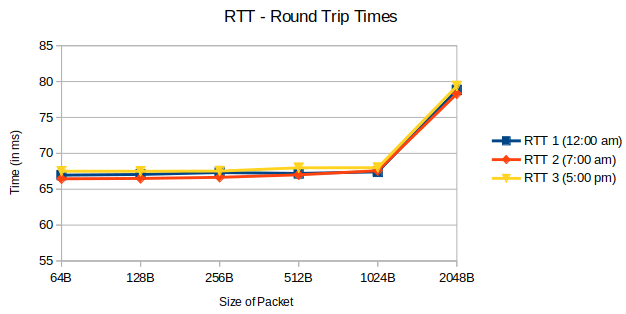
\includegraphics[width=12cm]{rtt2.png}
		\end{wrapfigure}
		\strut{}
		\textbf{RELATION BETWEEN RTT AND SIZE OF PACKET:-} It can be seen from the graph that the Round Trip Times(RTT) does not change much for smaller than equal to 1024 Bytes. After that there is a sudden noticeable jump in the RTT. This can be explained by the fact that \textbf{Maximum Transmission Unit} is 1500 Bytes by default. Smaller packets are padded to make 1500 Bytes. 2048B size packet is split into two parts. Hence RTT is almost the same for smaller than 1500 Bytes packets and increases for 2048 B packet as more packets are transmitted increasing the \textbf{transmission delay}.
	\end{adjustbox}
\end{enumerate}
\section*{Question 3}
\begin{enumerate}[a)]
	\item
	\rowcolors{1}{cyan!10}{cyan!20}
	\begin{tabularx}{0.95\textwidth}{|p{130pt}||X||X||X|}
		\hline
		\rowcolor{cyan!40}
		\textbf{Command} & \textbf{Packets Sent} & \textbf{Packets Recieved} & \textbf{Packets Loss Rate} \\ \hline
		 ping -n -c 1000 10.19.6.44 & 1000 & 1000 & 0\%\\ \hline
		ping -p ff00 -c 1000 10.19.6.44 & 1000 & 999  &0.1\% \\ \hline
	\end{tabularx}
	\item 
	\begin{tabularx}{0.95\textwidth}{|p{130pt}||X||X||X||p{90pt}|}
		\hline
		\rowcolor{cyan!40}
		\textbf{Command} & \textbf{Min Latency} & \textbf{Max Latency} & \textbf{Mean Latency} & \textbf{Median Latency} \\ \hline
		ping -n -c 1000 10.19.6.44 & 0.635ms & 1078ms & 54.5094ms & 37.8ms \\ \hline
		
		ping -p ff00 -c 1000 10.19.6.44 & 0.641ms & 1895ms & 61.8816ms & 30.9ms \\ \hline
	\end{tabularx}
	\item
	The histogram of ping latencies for both the commands is plotted
	\\
	\centering
	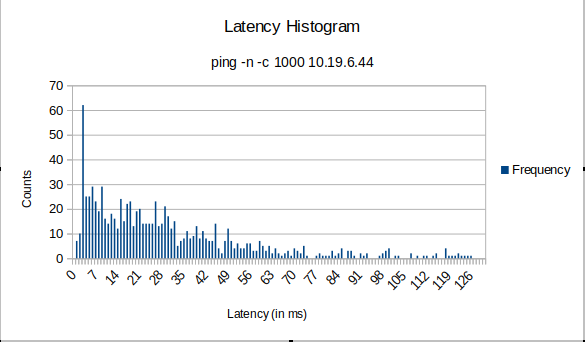
\includegraphics[width=12.5cm]{lat1.png}
	\\
	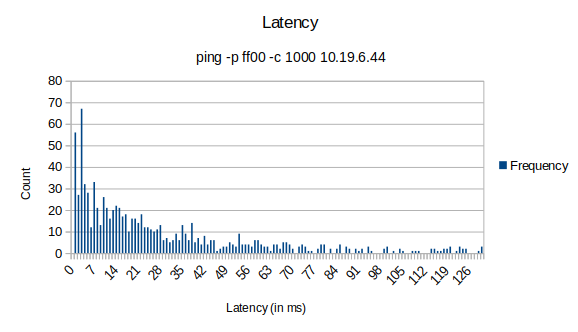
\includegraphics[width=13.5cm]{lat2.png}
	\\
	\flushleft
	From the histogram it is apparent that both the curves follow \textbf{Normal Distribution}.
	\item
	The mean latency is lower in the first command (that uses -n) as it makes no attempts to lookup symbolic names for host addresses and hence it is faster. Another difference between the two commands is that the second one (using -p ff00) is filled with 1111111100000000, therefore, has lower transitions in the signal that is sent. This is useful in checking data-dependent problems in the network. Since there are low transitions in the signal, clocking might become an issue especially for encodings that do do not use biphase encoding or scrambling techniques. Therefore it can be observed that the second command has a higher packet loss rate.
\end{enumerate}
\section*{Question 4}
\begin{enumerate}[a)]
	\item
	\begin{adjustbox}{valign=T,raise=\strutheight,minipage={\linewidth}}
		\begin{wrapfigure}{r}{0pt}
			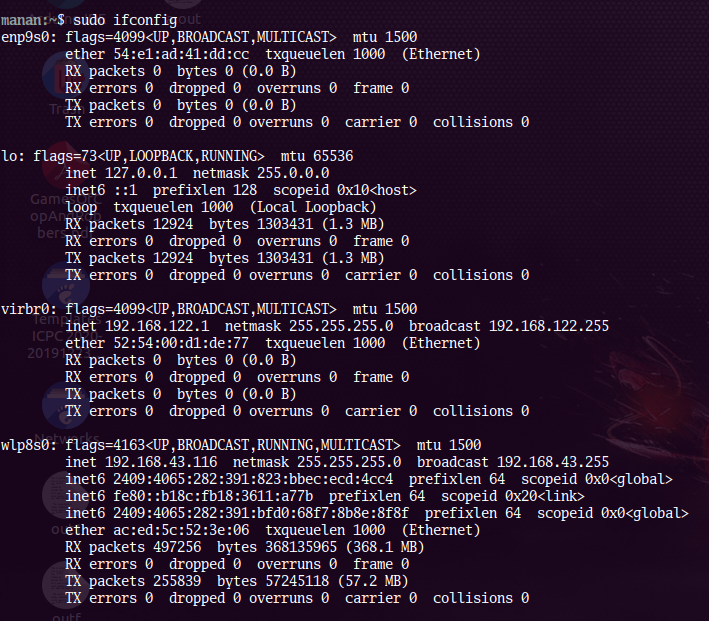
\includegraphics[width=10cm]{ifconfig.png}
		\end{wrapfigure}
		\strut{}
		\textbf{Inet} denotes the IP address of the machine, for \textbf{lo} it is the localhost. \textbf{broadcast} shows the broadcast address that is the address required to broadcast on the network connected through the interface of the machine. \textbf{Netmask} is used to divide IP address into subnets and specify the available hosts. Netmask defines how large a network is. \textbf{inet 6} refers to the IPv6 address.\textbf{UP} indicates that the server is configured to be enabled and \textbf{RUNNING} indicates that it is operational to accept data. \textbf{Multicast} indicates that the network can handle multicast packets. \textbf{MTU} (maximum transmission unit) is a link layer characteristic which provides the limit on the size of the ethernet frame. If an IP datagram is larger than the MTU then it is broken down into smaller pieces till each piece is in the range itself.The default value of MTU is 1500. \textbf{ether} shows the MAC address of the machine. \textbf{RX packets, Bytes} refer to the number of packets and bytes received respectively. \textbf{RX errors} refer to the number of damages packets received. \textbf{RX dropped} is the number of packets that were dropped. \textbf{RX frame} is the number of packets that experienced frame errors. similarly, \textbf{TX Packets} refers to the number of packets transmitted, \textbf{TX errors} refers to the number of packets that experienced errors. \textbf{txqueuelen} refers to the length of the transmission queue. \textbf{LOOPBACK} means that the interface is local loopback related.
	\end{adjustbox} 	
	\item 
	The options that can be applied with ifconfig interface are -
	\begin{itemize}
		\vspace{-0.25cm} \item \textbf{-a} it displays all the interfaces even if they are down
		\vspace{-0.2cm} \item \textbf{-s} it displays a short list
		\vspace{-0.2cm}\item \textbf{-v} it displays more verbose errors
		\vspace{-0.2cm}\item \textbf{mtu N} sets the MTU of an interface
		\vspace{-0.2cm}\item \textbf{down} causes the interface driver to be shut down
	\end{itemize}
	\item 
	\begin{adjustbox}{valign=T,raise=\strutheight,minipage={\linewidth}}
		\begin{wrapfigure}{l}{0pt}
			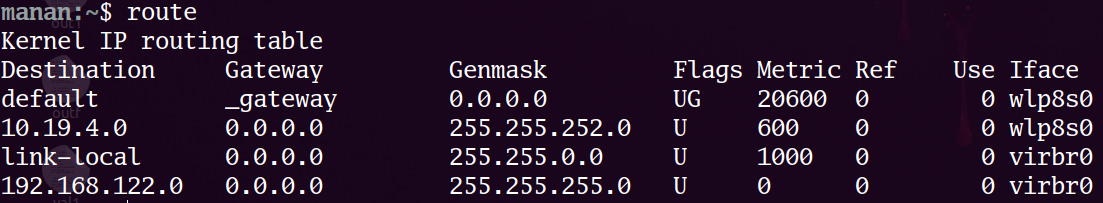
\includegraphics[width=10cm]{route1.png}
		\end{wrapfigure}
		\strut{}
		The \textbf{route} command is used to show the routing table of the device. The attached image shows the route command run locally. The \textbf{Destination} column shows the destination host or network. The \textbf{genmask} column represents the netmask of the network. The \textbf{gateway} column shows the gateway of the network. An asterisk in the field implies that no forwarding gateway is needed. \textbf{Iface} shows the network interfaces to which packets of this route will be sent. \textbf{Metric} is the distance of the target usually counted in hops. \textbf{G} flag means that the specified gateway should be used while the \textbf{U} flag shows that the network is up. \textbf{Ref} is the number of references to the route.
	\end{adjustbox} 
	
	\item 
	\begin{adjustbox}{valign=T,raise=\strutheight,minipage={\linewidth}}
		\begin{wrapfigure}{r}{0pt}
			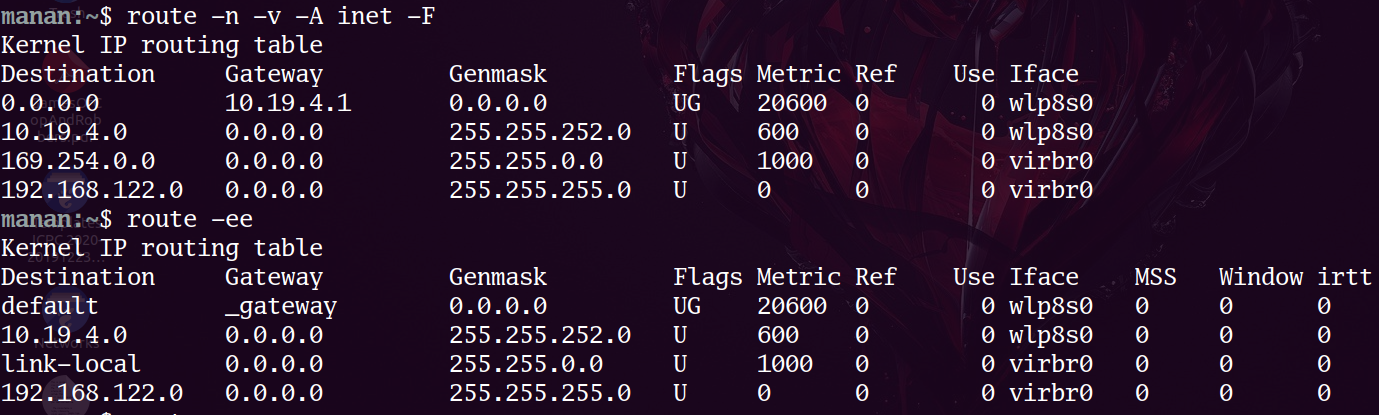
\includegraphics[width=10cm]{route2.png}
		\end{wrapfigure}
		\strut{}
		The options that can be applied with route are -
		\begin{itemize}
			\item \textbf{-n} it shows numerical IP addresses instead of determining symbolic host names
			\vspace{-0.2cm}\item \textbf{-F} it displays kernels FIB routing information
			\vspace{-0.5cm}\item \textbf{-ee} shows extra columns (MSS and Window) in the output
			\vspace{-0.2cm}\item \textbf{-v} to select verbose option
			\vspace{-0.2cm}\item \textbf{-A} to specify the address family
			\vspace{-0.2cm}\item \textbf{del} to delete a route
		\end{itemize}
	\end{adjustbox} 
	
\end{enumerate}

\section*{Question 5}
\begin{enumerate}[a)]
	\item \textbf{Netstat} is used to \textbf{print network connections, routing tables, interface statistics, masquerade connections, and multicast memberships}. It is one of the most basic command-line network utility tools and prints information about the Linux networking subsystem. It can be used for \textbf{performance measurement} and also to \textbf{find faults} in the network.
	\item 
	\begin{adjustbox}{valign=T,raise=\strutheight,minipage={\linewidth}}
		\begin{wrapfigure}{r}{0pt}
			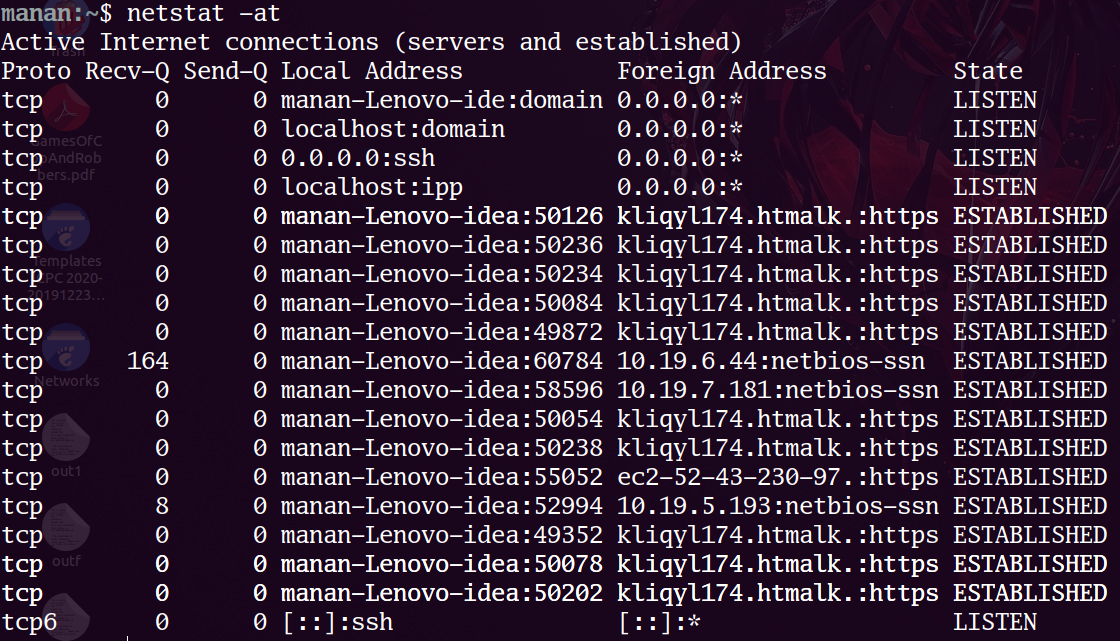
\includegraphics[width=10cm]{netstat1.png}
		\end{wrapfigure}
		\strut{}
		\textbf{netstat -at} is used to show all established TCP connections. \\
		The \textbf{Proto} column shows us whether the protocol is TCP or UDP. The amount of data in queue to be sent and read is shown by \textbf{Send-Q} and \textbf{Recv-Q} respectively. The \textbf{Local Address} and \textbf{Foreign Address} columns show the hosts and ports the listed sockets are connected to. The local end is the machine on which netstat is run, and the foreign end is the other computer. The \textbf{State} shows in which state the socket is in. eg - \textbf{LISTEN} (wait for some external computer to contact us) and \textbf{ESTABLISHED} (ready for communication).
	\end{adjustbox} 
	\item
	\begin{adjustbox}{valign=T,raise=\strutheight,minipage={\linewidth}}
		\begin{wrapfigure}{r}{0pt}
			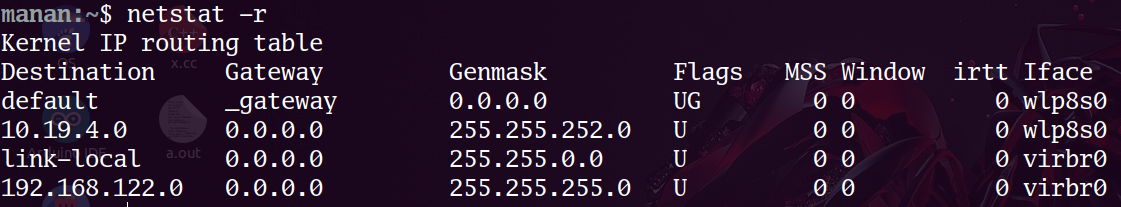
\includegraphics[width=10cm]{netstat2.png}
		\end{wrapfigure}
		\strut{}
		\textbf{netstat -r} shows the kernel routing table. The \textbf{Destination} column shows the destination host or network. The \textbf{genmask} column represents the netmask of the network. The \textbf{gateway} column shows the gateway of the network. \textbf{Iface} shows the network interfaces to which packets of this route will be sent. \textbf{G} flag means that the specified gateway should be used while the \textbf{U} flag shows that the network is up. \textbf{Ref} is the number of references to the route. The \textbf{MSS(Maximum Segment Size)} is the size of the	largest datagram the kernel can construct for transmission via this route. The \textbf{Window} is the maximum amount of data the system can accept in a single burst from a remote host. The acronym \textbf{irtt} is the initial round trip time. 0 in MSS and Window represents no changes from commonly used values.
	\end{adjustbox} 
	\item
	\begin{adjustbox}{valign=T,raise=\strutheight,minipage={\linewidth}}
		\begin{wrapfigure}{l}{0pt}
			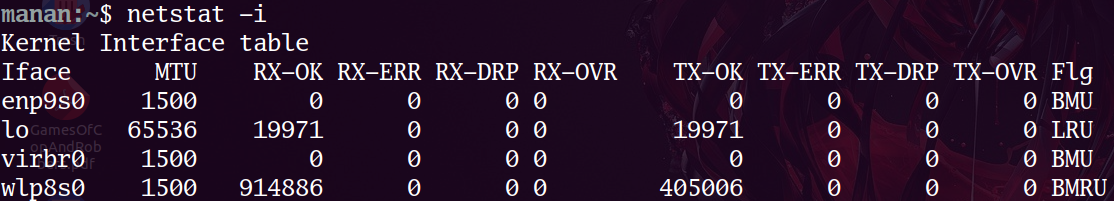
\includegraphics[width=10cm]{netstat3.png}
		\end{wrapfigure}
		\strut{}
		\textbf{netstat -i} is used to show the status of all the interfaces of the machine. \textbf{There are 4 interfaces on my computer.} \\
		The \textbf{Iface} column contains the name of the interface for which the statistics are shown. \textbf{MTU} is the value of Maximum Transmission Unit. \textbf{RX, TX} values represent the number of packets received and sent by the interface so far. \textbf{OK, ERR, DRP} and \textbf{OVR} stand for 'correctly received', 'received but with incorrect checksum', 'dropped because receive buffer was too full' and 'dropped because the kernel couldn’t get to it in time' respectively. Flags \textbf{B, M, L, U, R} stand for broadcast capability, multicast capability, loopback interface, up and running respectively.
	\end{adjustbox} 
	\begin{adjustbox}{valign=T,raise=\strutheight,minipage={\linewidth}}
		\begin{wrapfigure}{r}{0pt}
			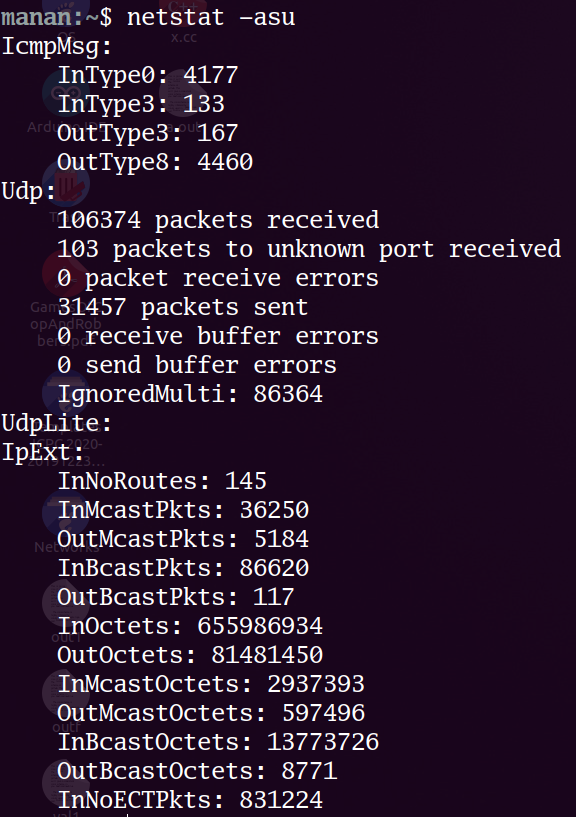
\includegraphics[width=7cm]{netstat5.png}
		\end{wrapfigure}
		\strut{}
		\item
		\textbf{netstat -asu} shows the statistics of all the UDP connections. The table fields are already described above.
		\item
		The \textbf{loopback} device/interface is a special, virtual network interface that the computer uses to communicate with itself. It is used for troubleshooting and diagnostics, and also to connect to servers running on the local machine. Consider the situation when a network interface is disconnected, then no communication on the interface is possible, not even the communication between the computer and itself. Loopback interface handles this problem by allowing applications running on the computer to connect to the servers on the same machine. It does not actually represent any hardware. For IPv4, the loopback interface is assigned all the IPs in the 127.0.0.0/8 address block (i.e.127.0.0.1 through 127.255.255.254).
	\end{adjustbox}
\end{enumerate}
\pagebreak
\section*{Question 6}
\textit{Time when the readings are taken are \textbf{12:00 am, 7:00 am, 5:00 pm. (Indian Standard Time)}}
\begin{table}[h]
	\rowcolors{1}{cyan!10}{cyan!20}
	\begin{tabularx}{\textwidth}{|p{100pt}||X||X||X||X||X||X|}
		\hline
		\rowcolor{cyan!40}
		  & \textbf{Youtube} & \textbf{Stanford} & \textbf{Codeforces} & \textbf{9anime} & \textbf{Hetzner} & \textbf{Sina Blog}\\ \hline
		\textbf{Hop Count 1} & 8 & 12 & 9 & 6 & 9 & 11 \\ \hline
		\textbf{Hop Count 2} & 8 & 12 & 9 & 6 & 9 & 11 \\ \hline
		\textbf{Hop Count 3} & 8 & 12 & 9 & 6 & 9 & 11 \\ \hline
	\end{tabularx}
	\caption{Round Trip Times for 6 hosts at 3 different times}
\end{table}
\begin{enumerate}[a)]
	\item The obvious common hop is the source of the packets. \textit{213.239.252.241} is a common hop for all. \textit{213.239.245.237} is a common hop for Stanford, Codeforces, 9anime and Hetzner. \textit{213.239.224.242} is a common hop between Codeforces and 9anime. Hops are common because the routes to the given destinations pass through some common internet circles and therefore overlap.
	\item Route to the same host might change during different times of the day due to \textbf{failure} on an intermediate path or because of \textbf{congestion} in that path. \textbf{Load balancing} is done to reduce the load of the congested path and therefore packets are redirected to routes having lower traffic. However, I did not experience any change in the path during the day.
	\item Sometimes \textit{traceroute} is unable to find the complete path to some hosts. This may happen because some servers/hosts on the route might not be configured to respond to the ICMP packet. Alternately, \textbf{firewalls} might also be setup that prevents responses and block ICMP traffic. It may also occur due to the \textbf{loss of packets} sent by the intermediate hosts.
	\item Yes, it is possible to find the route to certain hosts which fail to respond with ping experiment because both of them use different techniques. \textit{Ping} sends a packet to the specified address and expects a reply, relying on the \textbf{reply packet}. On the other hand, \textit{traceroute} works by sending packets with \textbf{TTL} (Time To Live) values that gradually increase from packet to packet. Routers decrement TTL values of packets by unit amount, discarding the ones which have reached 0 value, returning ICMP error. Thus \textit{traceroute} relies on \textbf{time exceeded packet}. Therefore the scenario can occur if the host blocks ICMP responses or has a firewall that does so.
\end{enumerate}
\section*{Question 7}
\begin{enumerate}[a)]
	\item
	\begin{adjustbox}{valign=T,raise=\strutheight,minipage={\linewidth}}
		\begin{wrapfigure}{l}{0pt}
			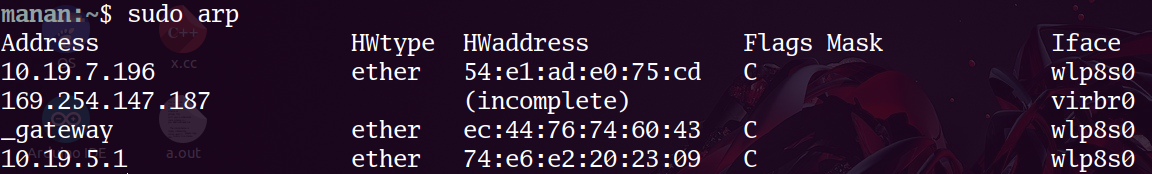
\includegraphics[width=10cm]{arp1.png}
		\end{wrapfigure}
		\strut{}
		\textbf{sudo arp} command is used to show the full arp (\textbf{Address Resolution Protocol}) table on the machine. The table is used to translate IP address to destination address on physical network. \textbf{Address} field shows the IP address. \textbf{HWaddress} shows the corresponding MAC address. \textbf{Mask} shows the netmask. \textbf{Iface} shows the interface name. \textbf{HWtype} tells the hardware type. \textbf{C} flag represents complete entries. \textbf{M} flag represents permanent entries.
	\end{adjustbox} 		
	\begin{adjustbox}{valign=T,raise=\strutheight,minipage={\linewidth}}
		\begin{wrapfigure}{r}{0pt}
			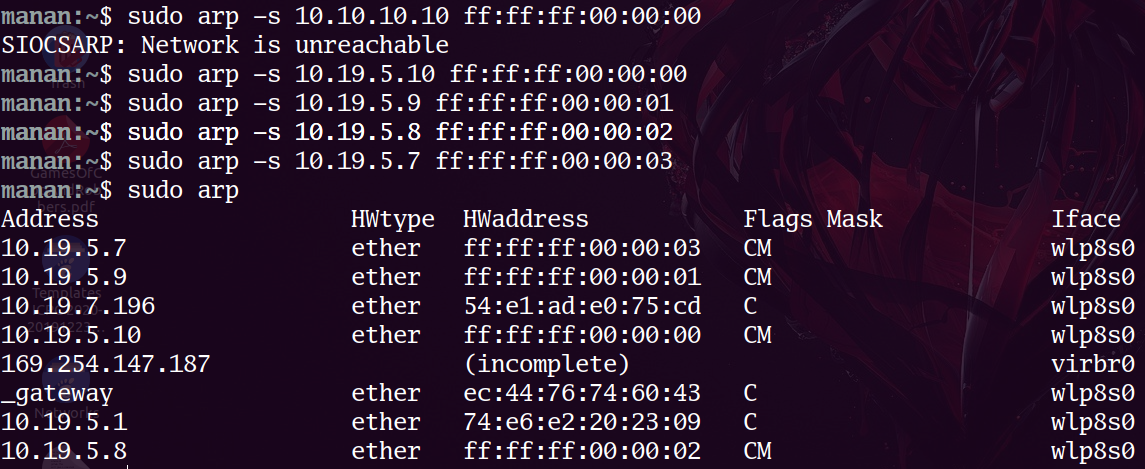
\includegraphics[width=8cm]{arp2.png}
		\end{wrapfigure}
		\strut{}
		\item
		\textbf{sudo arp -s (ipAddress) (MACaddress)} command is used to add entries into the arp table. \\
		\textbf{sudo arp -d (ipAddress)} command is used to delete entries into the arp table. \\
		It is not possible to add static entries for other subnets therefore the first command fails and the subsequent ones work.
		\item 
		\textbf{gc\_stale\_tim}e is the parameter that defines the amount of time the entries in the cache of the ARP module of the kernel remain valid. It can ve checked via the following command - \textbf{cat /proc/sys/net/ipv4/neigh/default/gc\_stale\_time}. The default value is \textbf{60 seconds}.
		\\
		A \textbf{trial and error} method to find this time would be to add a temporary entry and check after a fixed interval of time whether the entry is deleted or not. The time interval of checking can then be reduced for higher precision. \textbf{Binary search} technique can also be used.
		\item 
		It can occur that two IP addresses are mapped to the same Ethernet address in the case when a router or gateway connects two or more subnet ranges. MAC addressed is used while communicating within the same subnet range. In the ARP table, the IP addresses of the devices in other subnet ranges are mapped to the MAC/ethernet address of the router/gateway connecting those two subnets. Hence the ARP table contains the same ethernet address for the two IPs. The packet from this machine is sent to this router/gateway which sends the packet further to the correct device.
		\\
		\\
		One another situation that needs to be discussed here is that when two PCs with the same MAC address are connected within the same subnet mask. This situation howsoever unlikely is still possible. In such a situation the router will not send packets to either of the two IP's leading to a \textbf{100\% packet loss} in case they are pinged.
	\end{adjustbox} 
\end{enumerate}
\pagebreak
\section*{Question 8}
The following command is used. The analysis is done for \textbf{Lohit hostel}.
\\
\begin{center}
	\textbf{nmap -n -sP 10.19.4.1/22}
\end{center}
\textbf{subnet:} 10.19.4.1\\
\textbf{subnet mask:} 255.255.252.0\\
\begin{table}[h]
	\rowcolors{1}{cyan!10}{cyan!20}
	\begin{tabularx}{\textwidth}{|p{100pt}||X||X||X||X||X||X|}
		\hline
		\rowcolor{cyan!40}
		& \textbf{22:00:00} & \textbf{01:00:00} & \textbf{06:00:00} & \textbf{10:00:00} & \textbf{14:00:00} & \textbf{18:00:00}\\ \hline
		\textbf{Hosts Up} & 37 & 29 & 10 & 18 & 19 & 31 \\ \hline
	\end{tabularx}
	\caption{Number of Hosts up at different times}
\end{table}
\\
\begin{adjustbox}{valign=T,raise=\strutheight,minipage={\linewidth}}
	\begin{wrapfigure}{r}{0pt}
		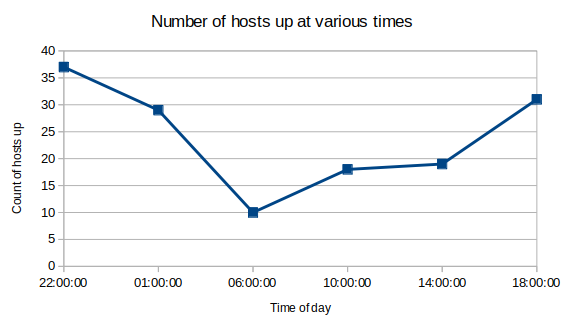
\includegraphics[width=12cm]{nmap.png}
	\end{wrapfigure}
	It is seen that most people are active during the night hours which seems consistent with the lifestyle of college students. The number of users decreases during early morning and then steadily rises till the evening.
	\\
	It seems that the numbers are a little low given that 1024 IP addresses are pinged. It is so because the hosts using Windows are not detected due to firewall which destroys the sent ICMP packets.
\end{adjustbox} 
\end{document}
